\subsection{Reducing the Size of a Mesh}
\label{sec:removing}


Meshes that are obtained by scanning real objects contain noise.
Most meshes that are generated by scanning require a complete
remeshing \cite{remeshing-2003}.
As a first step in remeshing, the curvature at each
vertex needs to be estimated.

In \cite{mmsb-2003}, Meyer et al., define the gaussian curvature operator
to estimate the curvature at each vertex. Their operator is 
based on the Gauss-Bonnet theorem.
The central idea is to cut a disk around each vertex that does not contain
any other vertices. Then, use the Gauss-Bonnet
to estimate the curvature in the removed
disk is occurs at the vertex of interest.

\todo{patch this in better}
We can combine our definition of discrete geodesic curvature
with the Gauss-Bonnet Theorem to obtain a formula for the discrete
curvature at a vertex.
To this end, consider a vertex in a triangulated surface.
We cut out this vertex, so that we obtain a topological disk containing
only the one vertex call this subsurface $M$. We have
$$\int_{\partial M}k_g=\sum_i\pi -(\gamma_i+\beta_{i+1})=\sum_i\alpha_i.$$
We now apply the Gauss-Bonnet Theorem.
The Euler characteristic of the disk is one and we know the geodesic curvature.
Thus, the discrete curvature at a vertex is given by
$\int_M K dA=2\pi-\sum_i\alpha_i$ and we define
the \EMPH{discrete Gaussian curvature} at a vertex $v$ to be

\begin{equation} \label{eqn:discrete-gaussian}
K(v):=2\pi -\sum_{f\in F_v}\alpha_f.
\end{equation}
\todo{make fig}


We associate an area around each vertex $v$. 
For each triangle incident to $v$, if the interior 
angle at $v$ is non-obtuse, mark the circumcenter of the triangle
and if the interior angle is obtuse, make the mid point of the edge
opposite of $v$. See \figref{mixed-area} for an illustration.
Denote the area of this polygon by $A_m.$
Since we are considering a closed disk $A$ we have $\chi(A)=1$.


\begin{figure}[htb]
\centering
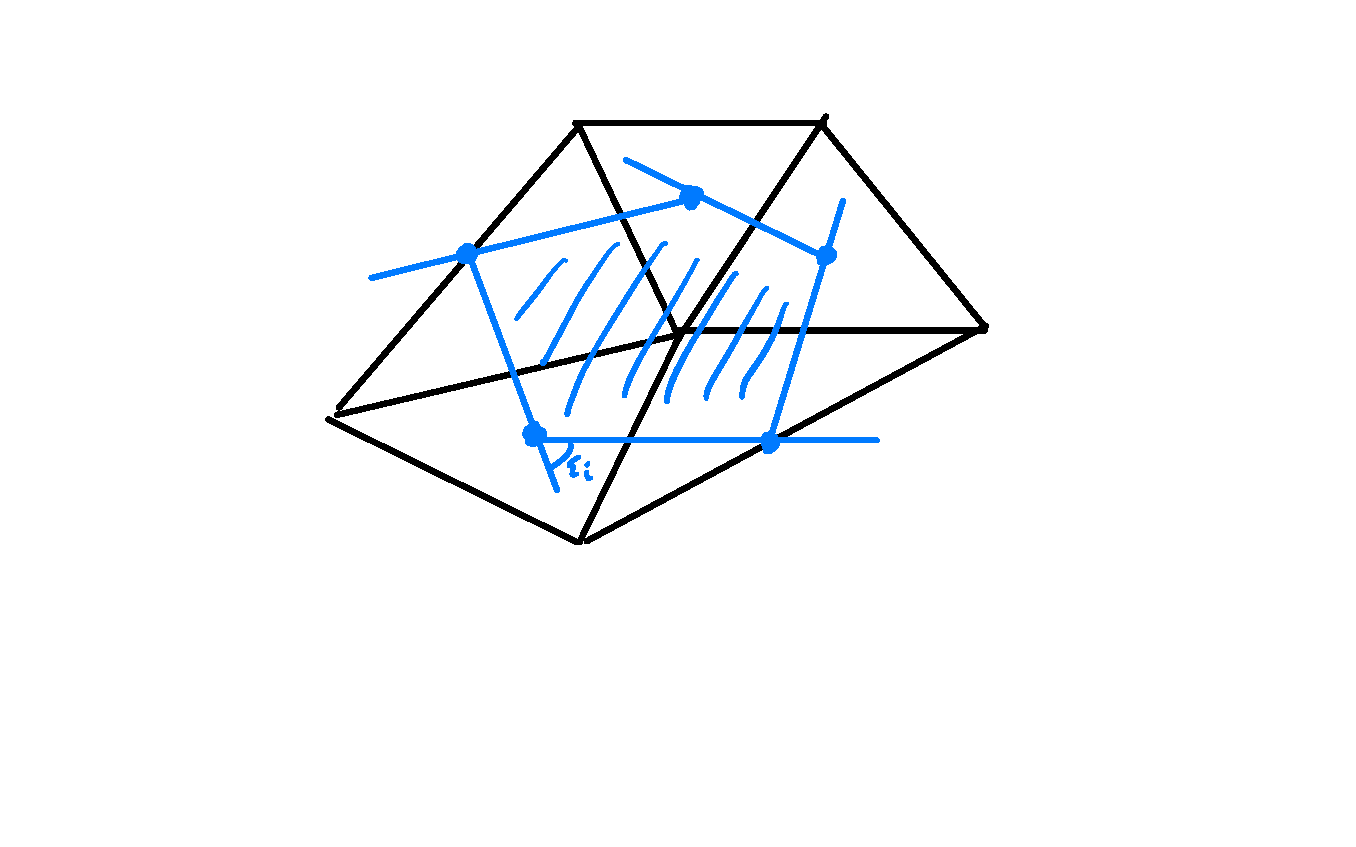
\includegraphics[width=.3\textwidth]{meshes/mixed-area}
\caption{The area $A_m$ associated with a vertex $v$.}
\label{fig:mixed-area}
\end{figure}

A continuous version of the Gauss-Bonnet Theorem
states that 
$$\int \int_{A_m}K dA +\sum_i^{F_v} \epsilon_i=2\pi.$$

Let $F_v$ denote the number of faces incident to $v$, 
then by the Gauss-Bonnet theorem we have


where the sum is over the faces incident to $v$.
The Gaussian curvature operator at a vertex $v$ is defined
to be
$$K(v)=\left( 2\pi -\sum_i^{F_v}\epsilon_i\right)/ A_m.$$

The experiments in \cite{mmsb-2003} found that the average
percent error did not exceed $1.3\%$ when using this operator.

Computing the curvature at each vertex in a mesh can allow one to reduce
the number of vertices in the mesh without sacrificing mesh quality.
This leads to more efficient algorithms and reduced storage space.
One example is given in \cite{alliez-2002},
Given a mesh, we compute the curvature at each vertex.
The number of points included in the re-mesh is determined
by the curvature. If the curvature is small, then few points
are sampled to be included in the re-mesh. If the curvature
is large, then many points are sampled. See \figref{planck-mesh}
for an illustration.

\begin{figure}[htb]
\centering
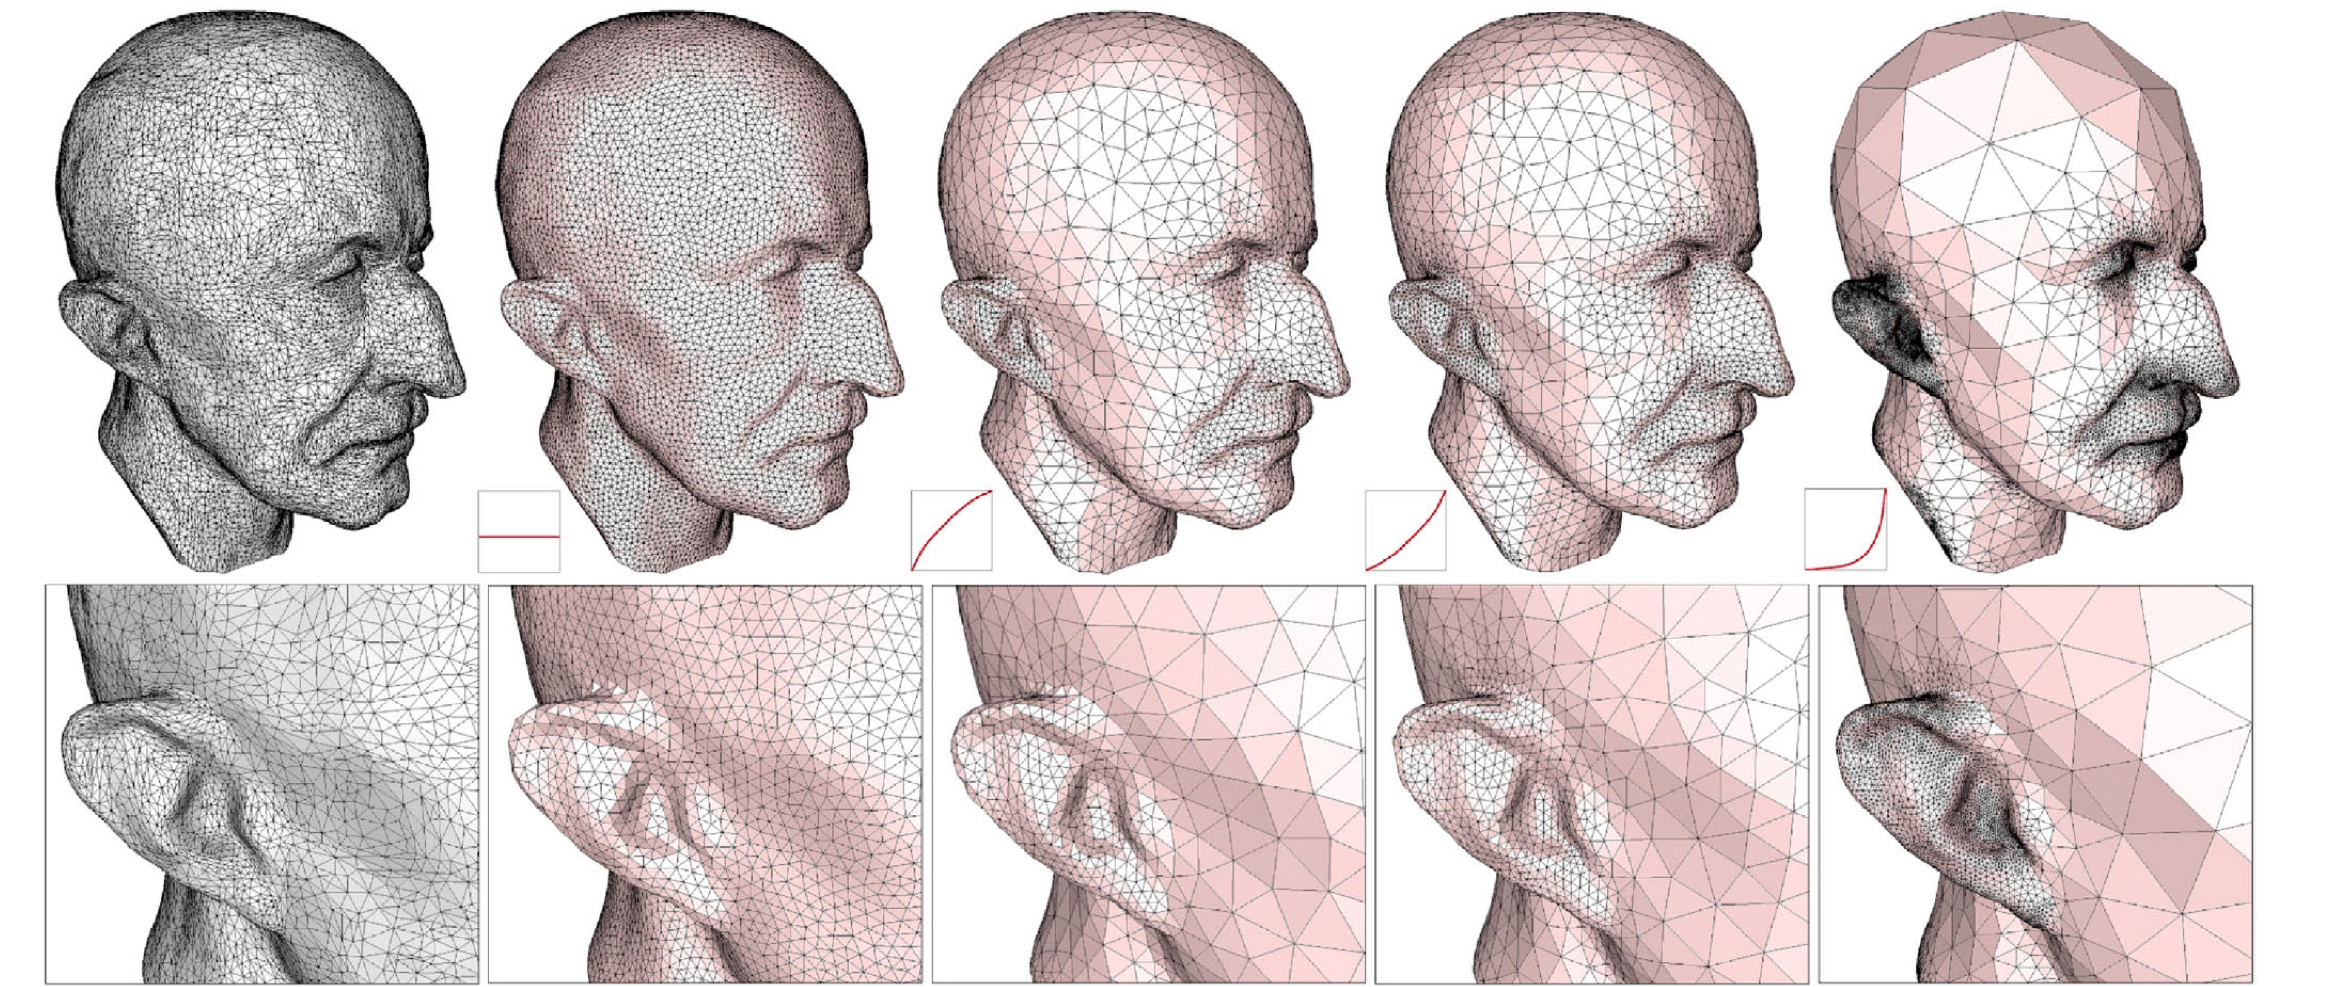
\includegraphics[width=.7\textwidth]{meshes/planck-mesh.jpeg}
\caption{A mesh of Max Plank. The original mesh is on the left. As we move
from left to right more importance is placed on vertices with large curvature.
Figure from \cite{alliez-2002}.}
\label{fig:planck-mesh}
\end{figure}